\documentclass[10pt,a4paper]{article}
\usepackage[utf8]{inputenc}\usepackage[T1]{fontenc}\usepackage[spanish,es-nodecimaldot]{babel}
\usepackage{lmodern,microtype}\usepackage[a4paper,margin=1.5cm,headheight=14pt]{geometry}
\usepackage{amsmath,amssymb,graphicx,booktabs,tabularx,longtable,array,xcolor,colortbl,caption,enumitem,fancyhdr,pdflscape,hyperref,needspace}
\definecolor{accent}{HTML}{174A6E}\hypersetup{colorlinks=true,linkcolor=accent,urlcolor=accent}
\setlength{\parindent}{0pt}\setlength{\parskip}{3pt}\setlength{\tabcolsep}{4pt}\renewcommand{\arraystretch}{1.15}
\setlist{nosep,leftmargin=*}\captionsetup{font=small,labelfont=bf}
\pagestyle{fancy}\fancyhf{}\fancyhead[L]{UNMSM -- FIEE}\fancyhead[R]{Microelectrónica y Sistemas Nanoelectrónicos | LD4}\fancyfoot[C]{\thepage}
\newcommand{\hojatitulo}[2]{\begin{center}{\Large\bfseries #1}\\[2pt]{\large #2}\\[3pt]Leonardo Sait Yactayo Tolentino (23190214) \quad Marco Antonio Arcila Santander (23190140)\\UNMSM -- Facultad de Ingeniería Electrónica y Eléctrica\\Docente: MsC. Luz Antuanet Adanaqué Infante \quad | \quad Semestre 2026-II\end{center}\vspace{-3pt}\hrule\vspace{5pt}}
\fancypagestyle{ldlandscape}{\fancyhf{}\fancyfoot[C]{\thepage}\renewcommand{\headrulewidth}{0pt}}
\newcommand{\ej}[1]{\needspace{3\baselineskip}\subsection*{#1}}
\addto\captionsspanish{\renewcommand{\tablename}{Tabla}}
\renewcommand{\thetable}{1.\arabic{table}}
\begin{document}
\renewcommand{\tablename}{Tabla}

\hojatitulo{Hoja de Control 1}{Modelo stuck-at y stuck-open}

\vspace{2pt}

\textbf{Convenciones:} vectores en orden $d\,c\,b\,a$ ($d=$ MSB); $V_{DD}=3{,}3\,\mathrm{V}$; umbral lógico $V_{th}=1{,}65\,\mathrm{V}$ ($V > 1{,}65\,\mathrm{V} \Rightarrow 1$). En la Tabla~\ref{tab:1.2}, $D=1/0$ denota valor sano/con fallo para \emph{s-a-0} y $\overline{D}=0/1$ para \emph{s-a-1}.

\ej{Ejercicio 1.1 -- Circuito sano y nudos de test}

\begin{figure}[ht]\centering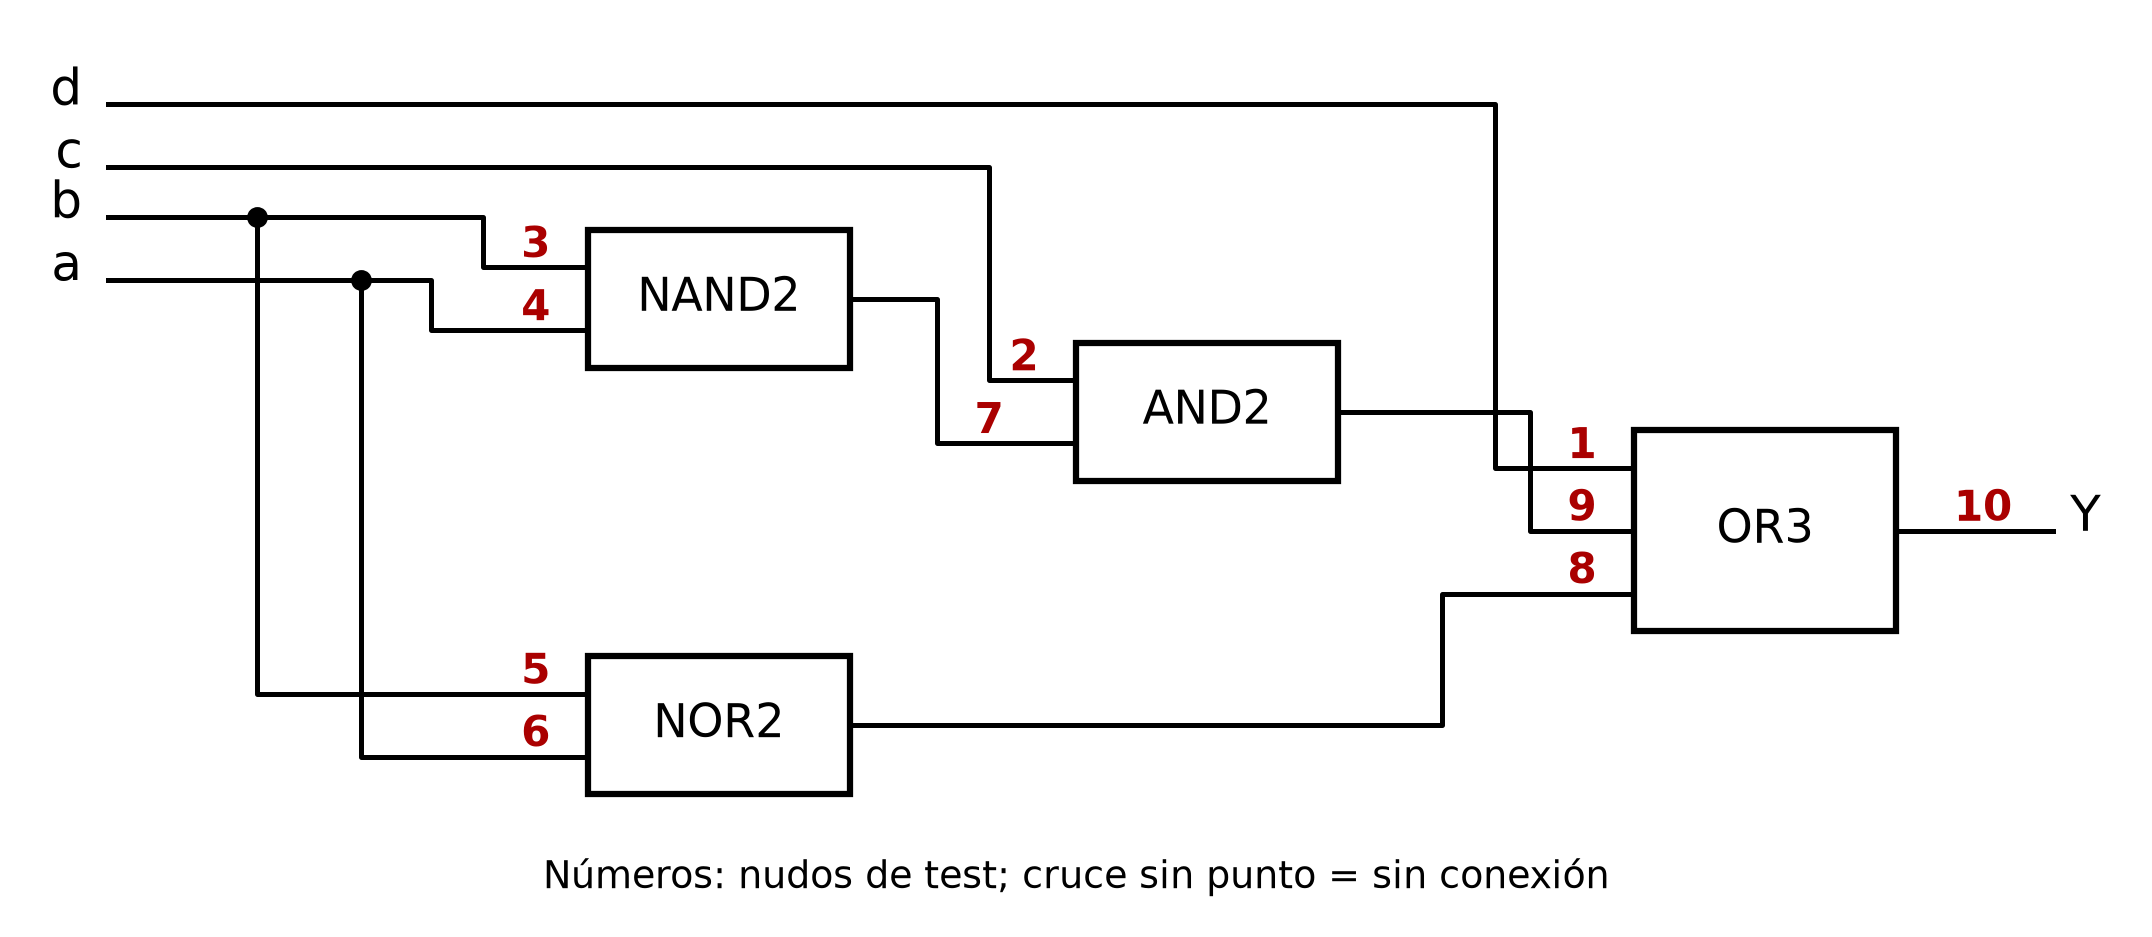
\includegraphics[width=.76\linewidth]{../figuras/esquema_nudos.png}\caption{Esquema lógico equivalente al netlist \texttt{P1\_segf\_stuckat.cir}. Los nudos 3 y 5 corresponden a ramas de \emph{fan-out} de $b$; los nudos 4 y 6, a ramas de \emph{fan-out} de $a$.}\label{fig:nudos}\end{figure}

\textbf{Función booleana:} $Y=d+c\overline{ba}+\overline{b+a}$. La compuerta NAND2 produce $\overline{ba}$ (nudo~7); AND2 calcula $c\overline{ba}$ (nudo~9); NOR2 calcula $\overline{b+a}$ (nudo~8); OR3 combina los tres términos hacia $Y$ (nudo~10). Como $b$ y $a$ presentan \emph{fan-out} $=2$ hacia NAND2 y NOR2, cada bifurcación física constituye un nudo de test independiente, totalizando 10 nudos y 20 fallos únicos.

\begin{table}[ht]\centering\caption{Salida del circuito sano (\texttt{NUDO=0}) medida en \texttt{P1\_segf\_stuckat.log}}\label{tab:1.1}\small
\begin{tabularx}{\linewidth}{>{\centering\arraybackslash}X>{\centering\arraybackslash}X>{\centering\arraybackslash}X>{\centering\arraybackslash}X>{\centering\arraybackslash}X>{\centering\arraybackslash}X}\toprule
Vector $d\,c\,b\,a$ & Dígito BCD & $Y$ teórica & $V(y)$ medido [V] & $Y$ lógico & ¿Coincide? \\ \midrule
0000 & 0 & 1 & 3,30 & 1 & Sí \\
0001 & 1 & 0 & 0,00 & 0 & Sí \\
0010 & 2 & 0 & 0,00 & 0 & Sí \\
0011 & 3 & 0 & 0,00 & 0 & Sí \\
0100 & 4 & 1 & 3,30 & 1 & Sí \\
0101 & 5 & 1 & 3,30 & 1 & Sí \\
0110 & 6 & 1 & 3,30 & 1 & Sí \\
0111 & 7 & 0 & 0,00 & 0 & Sí \\
1000 & 8 & 1 & 3,30 & 1 & Sí \\
1001 & 9 & 1 & 3,30 & 1 & Sí \\
1010 & --- & 1 & 3,30 & 1 & Sí \\
1011 & --- & 1 & 3,30 & 1 & Sí \\
1100 & --- & 1 & 3,30 & 1 & Sí \\
1101 & --- & 1 & 3,30 & 1 & Sí \\
1110 & --- & 1 & 3,30 & 1 & Sí \\
1111 & --- & 1 & 3,30 & 1 & Sí \\
\bottomrule\end{tabularx}\end{table}

\textbf{Secuencia lógica sana registrada:} \texttt{1000111011111111} (16/16 vectores coincidentes; $Y=1$ para los dígitos BCD $0,4,5,6,8,9$). \textbf{Retardo de propagación (cursores gráficos):} en la transición al vector $0001$, el cruce por $1{,}65\,\mathrm{V}$ ocurrió en $t_{V(a)}=10{,}050029\,\mathrm{ns}$ y $t_{V(y)}=10{,}088119\,\mathrm{ns}$, obteniendo $t_{pHL}=38{,}090\,\mathrm{ps}\approx 38{,}1\,\mathrm{ps}$ (lectura de cursores gráficos en LTspice, no directiva \texttt{.meas}).

\clearpage\pagestyle{ldlandscape}\begin{landscape}\ej{Ejercicio 1.2 -- D-algoritmo manual y verificación en LTspice}

Para \emph{s-a-0} se asigna $D=1/0$ y para \emph{s-a-1}, $\overline{D}=0/1$. La propagación hacia $Y$ por OR3 exige entradas laterales no controlantes $d=0$ y salida NOR2 $=0$ (salvo cuando el propio nudo~5 activa la propagación por NOR2, en cuyo caso requiere $a=0$ en NOR2 y salida AND2 $=0$).

\begin{table}[ht]\centering\caption{Activación, observación y justificación de control para los seis casos del D-algoritmo}\label{tab:1.2}\footnotesize
\begin{tabularx}{\linewidth}{>{\centering\arraybackslash}p{1.2cm}>{\centering\arraybackslash}p{2.3cm}>{\raggedright\arraybackslash}X>{\raggedright\arraybackslash}X>{\centering\arraybackslash}p{3.6cm}>{\centering\arraybackslash}p{3.0cm}}\toprule
Nudo & $D$ (fallo) & Observación: entradas laterales & Control: justificación & Vectores $d\,c\,b\,a$ & ¿Verificado en LTspice? \\ \midrule
7 & $D=1/0$ (\emph{s-a-0}) & $d=0$ y salida NOR2 $=0$; $c=1$ en AND2 & $\text{NAND2}=1 \Rightarrow ba\neq 11$; $\text{NOR2}=0 \Rightarrow (b,a)\neq(0,0)$ & 0101, 0110 & Sí (\texttt{Step 15}) \\
7 & $\overline{D}=0/1$ (\emph{s-a-1}) & $d=0$ y salida NOR2 $=0$; $c=1$ en AND2 & $\text{NAND2}=0 \Rightarrow b=a=1$ & 0111 & Sí (\texttt{Step 16}) \\
5 & $D=1/0$ (\emph{s-a-0}) & $a=0$ en NOR2; $d=0$ y salida AND2 $=0$ & $b=1$ activa; con $a=0$, $\text{NAND2}=1 \Rightarrow c=0$ & 0010 & Sí (\texttt{Step 11}) \\
5 & $\overline{D}=0/1$ (\emph{s-a-1}) & $a=0$ en NOR2; $d=0$ y salida AND2 $=0$ & $b=0$ activa; con $a=0$, $\text{NAND2}=1 \Rightarrow c=0$ & 0000 & Sí (\texttt{Step 12}) \\
9 & $D=1/0$ (\emph{s-a-0}) & $d=0$ y salida NOR2 $=0$ en OR3 & $\text{AND2}=1 \Rightarrow c=1, ba\neq 11$; $\text{NOR2}=0 \Rightarrow ba\neq 00$ & 0101, 0110 & Sí (\texttt{Step 19}) \\
9 & $\overline{D}=0/1$ (\emph{s-a-1}) & $d=0$ y salida NOR2 $=0$ en OR3 & $\text{AND2}=0$ con $\text{NOR2}=0 \Rightarrow ba\neq 00$ y $c\cdot\overline{ba}=0$ & 0001, 0010, 0011, 0111 & Sí (\texttt{Step 20}) \\
\bottomrule\end{tabularx}\end{table}\end{landscape}\clearpage\pagestyle{fancy}

\clearpage\pagestyle{ldlandscape}\begin{landscape}\ej{Ejercicio 1.3 -- Diccionario de fallos (\texttt{P1\_segf\_stuckat.log})}

Las 140 celdas (20 fallos únicos $\times$ 7 vectores oficiales) coinciden al 100\,\% con el barrido paramétrico de \texttt{P1\_segf\_stuckat.log} y \texttt{P1\_segf\_stuckat.raw}. Las celdas sombreadas difieren de la fila sana y detectan el fallo correspondiente.

\begin{longtable}{>{\centering\arraybackslash}p{3.4cm}*{7}{>{\centering\arraybackslash}p{2.35cm}}}\caption{Diccionario de fallos: salida lógica $Y$ por fallo y vector de test}\label{tab:1.3}\\\toprule
Fallo & 0101 & 0111 & 0000 & 0001 & 0010 & 0110 & 1010 \\ \midrule
\endfirsthead
\toprule
Fallo & 0101 & 0111 & 0000 & 0001 & 0010 & 0110 & 1010 \\ \midrule
\endhead
Sin fallo (\texttt{NUDO=0}) & 1 & 0 & 1 & 0 & 0 & 1 & 1 \\
1 / s-a-0 & 1 & 0 & 1 & 0 & 0 & 1 & \cellcolor{accent!18}0 \\
1 / s-a-1 & 1 & \cellcolor{accent!18}1 & 1 & \cellcolor{accent!18}1 & \cellcolor{accent!18}1 & 1 & 1 \\
2 / s-a-0 & \cellcolor{accent!18}0 & 0 & 1 & 0 & 0 & \cellcolor{accent!18}0 & 1 \\
2 / s-a-1 & 1 & 0 & 1 & \cellcolor{accent!18}1 & \cellcolor{accent!18}1 & 1 & 1 \\
3 / s-a-0 & 1 & \cellcolor{accent!18}1 & 1 & 0 & 0 & 1 & 1 \\
3 / s-a-1 & \cellcolor{accent!18}0 & 0 & 1 & 0 & 0 & 1 & 1 \\
4 / s-a-0 & 1 & \cellcolor{accent!18}1 & 1 & 0 & 0 & 1 & 1 \\
4 / s-a-1 & 1 & 0 & 1 & 0 & 0 & \cellcolor{accent!18}0 & 1 \\
5 / s-a-0 & 1 & 0 & 1 & 0 & \cellcolor{accent!18}1 & 1 & 1 \\
5 / s-a-1 & 1 & 0 & \cellcolor{accent!18}0 & 0 & 0 & 1 & 1 \\
6 / s-a-0 & 1 & 0 & 1 & \cellcolor{accent!18}1 & 0 & 1 & 1 \\
6 / s-a-1 & 1 & 0 & \cellcolor{accent!18}0 & 0 & 0 & 1 & 1 \\
7 / s-a-0 & \cellcolor{accent!18}0 & 0 & 1 & 0 & 0 & \cellcolor{accent!18}0 & 1 \\
7 / s-a-1 & 1 & \cellcolor{accent!18}1 & 1 & 0 & 0 & 1 & 1 \\
8 / s-a-0 & 1 & 0 & \cellcolor{accent!18}0 & 0 & 0 & 1 & 1 \\
8 / s-a-1 & 1 & \cellcolor{accent!18}1 & 1 & \cellcolor{accent!18}1 & \cellcolor{accent!18}1 & 1 & 1 \\
9 / s-a-0 & \cellcolor{accent!18}0 & 0 & 1 & 0 & 0 & \cellcolor{accent!18}0 & 1 \\
9 / s-a-1 & 1 & \cellcolor{accent!18}1 & 1 & \cellcolor{accent!18}1 & \cellcolor{accent!18}1 & 1 & 1 \\
10 / s-a-0 & \cellcolor{accent!18}0 & 0 & \cellcolor{accent!18}0 & 0 & 0 & \cellcolor{accent!18}0 & \cellcolor{accent!18}0 \\
10 / s-a-1 & 1 & \cellcolor{accent!18}1 & 1 & \cellcolor{accent!18}1 & \cellcolor{accent!18}1 & 1 & 1 \\ \midrule
Fallos detectados por vector & 5 & 7 & 4 & 6 & 6 & 5 & 2 \\
\bottomrule\end{longtable}\end{landscape}\clearpage\pagestyle{fancy}

\ej{Ejercicio 1.4 -- Cobertura acumulada y comparación de conjuntos}

\begin{table}[ht]\centering\caption{Cobertura acumulada de fallos únicos (sin doble conteo de $10/\text{s-a-0}$)}\label{tab:1.4}\scriptsize
\begin{tabularx}{\linewidth}{>{\centering\arraybackslash}p{1.0cm}>{\centering\arraybackslash}p{1.9cm}>{\raggedright\arraybackslash}X>{\centering\arraybackslash}p{1.7cm}>{\centering\arraybackslash}p{1.7cm}>{\centering\arraybackslash}p{1.7cm}}\toprule
Orden & Vector $d\,c\,b\,a$ & Fallos nuevos detectados & N.º nuevos & Acumulado & Cobertura \\ \midrule
1 & 0101 & 2/s-a-0, 3/s-a-1, 7/s-a-0, 9/s-a-0, 10/s-a-0 & 5 & 5 & 25\,\% \\
2 & 0111 & 1/s-a-1, 3/s-a-0, 4/s-a-0, 7/s-a-1, 8/s-a-1, 9/s-a-1, 10/s-a-1 & 7 & 12 & 60\,\% \\
3 & 0000 & 5/s-a-1, 6/s-a-1, 8/s-a-0 & 3 & 15 & 75\,\% \\
4 & 0001 & 2/s-a-1, 6/s-a-0 & 2 & 17 & 85\,\% \\
5 & 0010 & 5/s-a-0 & 1 & 18 & 90\,\% \\
6 & 0110 & 4/s-a-1 & 1 & 19 & 95\,\% \\
7 & 1010 & 1/s-a-0 & 1 & 20 & 100\,\% \\
\bottomrule\end{tabularx}\end{table}

\begin{table}[ht]\centering\caption{Comparación de conjuntos de vectores sobre el diccionario completo de 16 vectores}\label{tab:1.5}\scriptsize
\begin{tabularx}{\linewidth}{>{\raggedright\arraybackslash}p{3.9cm}>{\centering\arraybackslash}p{1.9cm}>{\centering\arraybackslash}p{1.9cm}>{\centering\arraybackslash}p{1.6cm}>{\raggedright\arraybackslash}X}\toprule
Conjunto & N.º vectores & Fallos det. & Cobertura & Fallos no detectados \\ \midrule
Optimizado (Tabla~\ref{tab:1.4}) & 7 & 20 & 100\,\% & Ninguno \\
Funcional: BCD (0000--1001) & 10 & 20 & 100\,\% & Ninguno \\
Aleatorio: 1100, 0011, 1001, 0110 & 4 & 10 & 50\,\% & 2/s-a-1, 3/s-a-0, 3/s-a-1, 4/s-a-0, 5/s-a-0, 5/s-a-1, 6/s-a-0, 6/s-a-1, 7/s-a-1, 8/s-a-0 \\
\bottomrule\end{tabularx}\end{table}

La progresión correcta es 25\,\%, 60\,\%, 75\,\%, 85\,\%, 90\,\%, 95\,\% y 100\,\%. El fallo $10/\text{s-a-0}$ ya es detectado por $0101$ y no vuelve a contarse en $0000$; el séptimo vector ($1010$) detecta por primera vez $1/\text{s-a-0}$.

\ej{Ejercicio 1.5 -- Fallo stuck-open (\texttt{P1\_stuckopen.cir})}

En \texttt{P1\_stuckopen.cir} se intercala $R_{SO}$ ($1\,\mathrm{m}\Omega$ sano; $1\,\mathrm{T}\Omega$ abierto) en el drenaje del NMOS de entrada $a$ de \texttt{NOR2\_SO}. En $T_0=0000$ el nudo $o8$ se precarga a $3{,}30\,\mathrm{V}$; en $T_1=0001$ ($b=0,a=1$), la red pull-up queda cortada y el drenaje de $MNA$ abierto, por lo que $o8$ flota reteniendo nivel alto ($Y=1$ frente a $0$ sano, detectando el fallo). En $T_2=0011$, el NMOS sano de $b$ descarga $o8$ a $0\,\mathrm{V}$; al volver a $0001$ en $T_3$, $o8$ vuelve a flotar descargado ($Y=0$) y no detecta el defecto.

\begin{table}[ht]\centering\caption{Ensayo \emph{stuck-open} en \texttt{NOR2\_SO}: muestras \texttt{.meas} a $t=8, 18, 28, 38\,\mathrm{ns}$ (\texttt{P1\_stuckopen.log})}\label{tab:1.6}\small
\begin{tabularx}{\linewidth}{>{\centering\arraybackslash}p{1.0cm}>{\centering\arraybackslash}p{1.9cm}>{\centering\arraybackslash}X>{\centering\arraybackslash}p{1.5cm}>{\centering\arraybackslash}X>{\centering\arraybackslash}p{1.9cm}>{\centering\arraybackslash}p{1.6cm}}\toprule
Paso & Vector $d\,c\,b\,a$ & $V(o8)$ sano [V] & $Y$ sano & $V(o8)$ \emph{stuck-open} [V] & $Y$ \emph{stuck-open} & ¿Detecta? \\ \midrule
T0 & 0000 & 3,30 & 1 & 3,30 & 1 & No \\
T1 & 0001 & 0,00 & 0 & 3,45 & 1 & Sí \\
T2 & 0011 & 0,00 & 0 & 0,00 & 0 & No \\
T3 & 0001 & 0,00 & 0 & $-0{,}11$ & 0 & No \\
\bottomrule\end{tabularx}\end{table}

\textbf{Muestras estables vs.\ extremos transitorios (\texttt{P1\_stuckopen.raw}):} en la corrida $R_{SO}=1\,\mathrm{T}\Omega$, las muestras \texttt{.meas} registran $V(o8)=3{,}450976\,\mathrm{V}$ ($T_1$, $18\,\mathrm{ns}$) y $-0{,}114028\,\mathrm{V}$ ($T_3$, $38\,\mathrm{ns}$), mientras que en el trazado transitorio continuo se observan máximos de $3{,}451\,\mathrm{V}$ a $10{,}120\,\mathrm{ns}$ ($T_1$) y un pico inicial de $3{,}811\,\mathrm{V}$ a $20{,}045\,\mathrm{ns}$ ($T_2$, antes de la descarga por $MNB$), así como un mínimo transitorio de $-0{,}144\,\mathrm{V}$ a $30{,}100\,\mathrm{ns}$ ($T_3$) que relaja a $-0{,}114\,\mathrm{V}$ antes de $38\,\mathrm{ns}$. Estos desplazamientos fuera de $[0;\,3{,}3]\,\mathrm{V}$ son coherentes con el acoplamiento capacitivo (\emph{feedthrough}) a través de las capacidades de solapamiento puerta-drenador de \texttt{NOR2\_SO} sobre un nudo de alta impedancia en $R_{SO}=1\,\mathrm{T}\Omega$. \textbf{Número de vectores necesarios:} se requiere una pareja ordenada de \textbf{2 vectores} ($0000 \to 0001$). El conjunto de 7 vectores de la Tabla~\ref{tab:1.4} \textbf{sí detecta} este \emph{stuck-open}, ya que sus vectores 3.º (\texttt{0000}) y 4.º (\texttt{0001}) se aplican en el orden requerido.

\textbf{Conclusiones del grupo:} (1) Los siete vectores optimizados detectan el 100\,\% de los veinte fallos únicos \emph{stuck-at}. (2) El D-algoritmo permite justificar analíticamente cada vector y verificarlo bit a bit contra el registro SPICE. (3) El fallo \emph{stuck-open} exige parejas ordenadas de inicialización y prueba ($0000 \to 0001$) debido a la retención capacitiva en el nudo flotante.

\end{document}
